\documentclass[ngerman]{article}

% Add all packages here
\usepackage[utf8]{inputenc}
\usepackage{amsmath, amsthm, amsfonts, amssymb}
\usepackage[margin=1in]{geometry}

% Useful custom commands I like. Feel free to send a PR :=)

% all number domains
\newcommand{\N}{\mathbb{N}}
\newcommand{\Z}{\mathbb{Z}}
\newcommand{\R}{\mathbb{R}}
\newcommand{\C}{\mathbb{C}}

% short versions of math arrows
\newcommand{\larr}{\leftarrow}
\newcommand{\rarr}{\rightarrow}
\newcommand{\lrarr}{\leftrightarrow}
\newcommand{\Larr}{\Leftarrow}
\newcommand{\Rarr}{\Rightarrow}
\newcommand{\Lrarr}{\Leftrightarrow}

% You can also just overshadow them by overwriting in the main.tex file
\title{Automatisierte Generation von Anki-basierten Karteikarten aus Markdownquellen}
\author{Lars Quentin\\Beteuung: Prof. Dr. Carsten Damm}
\date{03.03.2023}


\begin{document}
\maketitle
% ABSTRACT
\section*{Abstract}
Karteikarten und selbstgeschriebene Zusammenfassungen sind zwei wertvolle Ressourcen zur Vorbereitung von Klausuren und dem generellen Lernen neuer Themenbereiche. Während Karteikarten sich am besten für wissensintensives Auswendiglernen eignen sind Zusammenfassungen besser zum Verstehen komplexer, stark zusammenhängender Themen. Das Ziel dieser Arbeit liegt darin, diese beiden Ansätze zu vereinen. Durch die Konzipierung einer Markdownerweiterung mit Karteikartensyntax wurde die Möglichkeit geschaffen, aus Zusammenfassungen Karteikartendecks zu extrahieren, welche dann isoliert mit dem Spaced-Repitition-System Anki gelernt werden können. Des weiteren wurden für GitHub sowie GitLab kollaborative Workflows entwickelt, bei welchem automatisiert nach jedem Commit durch die Nutzung von Continuous Integration (CI) automatisiert ein neues Kartenarchiv erstellt wird.
\tableofcontents
\newpage


\section{Einführung}
\subsection{Motivation}
Das Problem des Lernens, insbesondere in universitären Bereich, lässt sich in zwei distinkte Kategorien aufteilen: Das verständnisorienterte Lernen komplexer Themen und das faktenbasierte Lernen spezifischer Details. Obwohl die meisten Klausuren eine Kombination beider Kategorien darstellen, erfordert jede Art unterschiedliche Vorgehensweisen:

\begin{itemize}
\item Im Falle verständnisbasierter komplexer Themen können Lernzettel geschrieben werden, in dem Informationen zusammengefasst und strukturiert werden. Dies resultiert in immer noch großen komplexen Texten oder Stichpunktlisten, in welchen die einzelnen Informationen sehr zusammenhängend sind. Die einzelnen Themen sind weniger isoliert; das erwartete Detailwissen ist geringer. Diese Klasse an Themen ist typisch für logisch-orientierte Studiengänge wie z.B. Mathematik, Philosophie, Informatik oder Physik.
\item Im Gegensatz dazu erfordert das akribische Lernen von faktenbasierten Details viel Auswendiglernen und wird meistens über Karteikarten praktiziert. Dieser Ansatz ist typisch für Studiengänge mit einem hohen Lernvolumen, wie z.B. Medizin, Biologie oder Sprachwissenschaften. Allgemein findet sich diese Problemart oft in komplexen, nicht-menschengemachten Systemen wieder.
\end{itemize}

Im digitalen Bereich gibt es für diese beide Arten des Klausurlernens kanonische Lösungen:
\begin{itemize}
  \item \textbf{Lernzettel:} Insbesondere in der Informatik werden für Lernzettel immer häufiger Markdown \cite{Markdown} verwendet. Markdown ist eine einfache, aber leistungsstarke Markup-Sprache die einige Vorteile bietet: Zum einen kann sie ohne spezielle Software direkt von Menschen geschrieben werden, zum anderen ist sie einfach parsebar, wodurch sie mit vielen Tools genutzt werden kann. Zudem kann Markdown durch die simple, zeilenbasierte Struktur mit Git versioniert werden. Es unterstützt simple Medien wie Tabellen, Bilder und \LaTeX-Formeln, was es für die meisten Anwendungsfälle expressiv genug macht. Es gibt auch Tools wie Hedgedoc \cite{HedgeDoc} zum kollaborativen Live-Editieren, welches unter anderem auch als Instanz von der GWDG gehosted wird \cite{HedgeDocGWDG}. Es ist einfach, Markdown durch Applikationen wie Pandoc \cite{Pandoc} in HTML oder RevealJS-Presentationsfolien \cite{RevealJS} via Hedgedoc zu exportieren.
  \item \textbf{Karteikarten:} Digitale Karteikarten werden häufig mit sogenannten Spaced-Repitition-Systemen (SRS) gelernt. Ein SRS ist ein Lernsystem, das Lernaufwand minimiert, indem es die optimale Zeit zur nächsten Wiederholung der Frage auf Basis der bisherigen Kartenhistorie sowie der Selbsteinschätzung der Schwierigkeit approximiert. Dies bedeutet das Fragen, die man leicht beantworten kann, seltener wiederholt werden als schwierigere Fragen, mit welchen man auch historisch bereits Probleme hatte.\\
    Das bei weitem beliebteste SRS ist Anki \cite{Anki}, ein Open-Source-Programm \cite{AnkiGithub}, das durch eine iOS-App \cite{AnkiiOS} finanziert wird. Es basiert auf Chromium \cite{QTWebEngine} und hat somit einen hohen Mediensupport. Anki bietet einen kostenlosen Cloud-Sync \cite{AnkiCloud}, der es ermöglicht, Karteikarten auf verschiedenen Geräten zu synchronisieren. Darüber hinaus gibt es eine kostenlose, von der Community erstellte Androidversion. Anki hat auch eine große Bibliothek von Decks, die von der Community geteilt werden, sowie Plug-Ins-Support \cite{AnkiPlugins}, die es Benutzern ermöglicht, die Funktionalität von Anki zu erweitern.
\end{itemize}

Trotz der Vorteile, die sowohl Lernzettel als auch Karteikarten bieten, haben sie jeweils auch ihre Nachteile. Lernzettel sind ineffizient zum Details lernen, da sie oft sehr verbos sind und eine geringere Informationsdichte haben. Darüber hinaus kann man keinen expliziten Fokus auf Themen setzen, welche einem besonders schwerfallen, da der Text sich nicht so einfach in atomare Fakten aufteilen lässt. Karteikarten jedoch verlieren schnell ihre Reihenfolge. Zudem kann man zwischen Karteikarten keinen Kontext erhalten, welcher gegebenenfalls benötigt wird um das größere Konzept zu verstehen.

\newpage

In diesem Praktikumsbericht wird eine Lösung vorgestellt, Lernzettel mit Markdown und Karteikarten mit Anki logisch zu verbinden. Die Idee basiert auf dem Konzept von Literate Programming.\\

Literate Programming ist ein Konzept, das von Donald E. Knuth entwickelt wurde \cite{LitProg}. Es kombiniert Programmcode mit dessen Dokumentation, so dass beide in einer einzelnen Datei vereint werden. Die Funktionen sind innerhalb der Dokumentation integriert und die gesamte Dokumentation lässt sich ausführen. Das ursprüngliche Konzept von Literate Programming verwendet eine eigene Sprache namens "WEB", welche von Knuth selbst entwickelt wurde. WEB-Quelldateien kompilierten entweder zu Pascal oder \TeX \cite{WebIntroduction}.\\

Moderne Umsetzungen von Literate Programming sind Jupyter Notebooks \cite{Jupyter}. Jupyter Notebooks sind interaktive Dokumente, die Code, Markdowntext und Medien durch sogenannte Zellen in einem Dokument vereinigen. Da Jupyter Notebooks ohne explizite Programmierumgebung gehosted in einem Webbrowser, zum Beispiel via GWDG Jupyter Hub \cite{JupyterGWDG} oder Google Colab \cite{Colab}, benutzbar sind haben sie eine geringe Einstiegshürde. Hierdurch sind sie interdisziplinär in der Forschung omnipräsent. Sie implementieren das Konzept von Literate Programming, indem man den Code als Teil des Dokumentes betrachtet statt als isolierte Einheit.

\subsection{Ziele und Beitr\"age}
Das Ziel dieser Arbeit ist, analog zum Konzept des Literate Programming, Karteikarten in Markdownzusammenfassungen zu integrieren. Hierdurch wird es möglich, das gesamte Markdown-Ökosystem zum Erstellen, Bearbeiten und Versionieren der Karteikarten zu nutzen. Einerseits ermöglicht dies, dass Karteikarten den Kontext und die Reihenfolge behalten, welche für das Lernen komplexer Themen erforderlich ist. Andererseits soll ein automatischer Anki-Export ermöglicht werden, der die Nutzung von Spaced Repitition für ein effizienteres Lernen von Fakten ermöglicht.\\

Im Rahmen dieses Praktikums wurden mehrere Beiträge geleistet, um die gesteckten Ziele zu erreichen. Zunächst wurde ein neuer Dateistandard für \texttt{.anki.md} Dateien entwickelt, um die Integration von Karteikarten in Markdownzusammenfassungen zu ermöglichen.

Darüber hinaus wurde ein Tool erstellt, das automatisch aus einem Ordner mit Markdown-Dateien ein Ankideck erstellen kann \cite{Ankiding}. Hierbei wird die Ordnerstruktur auf die Struktur der Ankidecks übertragen, und es wird sämtliche Markdown Syntax sowie das Rendering von \LaTeX-Formeln unterstützt. Das Tool kann auch mit der Mobilversion von Anki genutzt werden. Zudem kann mit dem Ankideck offline gelernt werden, da alle verlinkten Bilder in das Deckarchiv gespeichert werden.\\

Zuletzt wurden Git-Repository-Vorlagen für GitLab \cite{GitlabTemplate} und GitHub \cite{GithubTemplate} konzipiert und implementiert, mit welchen automatisch via Continuous Integration nach jedem Commit ein aktualisiertes Ankideckarchiv erstellt wird. Dies ermöglicht die Erschaffung von Ankikarten ohne lokal installierte oder technischem Verständnis des Konvertierungsprozesses.

\newpage


\section{Softwarekonzeptionierung und Methodologie}
\subsection{Entwurf einer Markdownerweiterung}
Markdown ist zwar sehr verbreitet, jedoch gibt es keine universale Markdownspezifikation. Stattdessen gibt es viele verschiedene Varianten, welche aber leicht voneinander abweichen. Somit, bevor man einen Markdownstandard erweitern kann, muss ein Grundstandard spezifiziert werden.

Für den Anwendungsfall dieses Praktikums wird als Basis der am weitesten verbreite CommonMark \cite{CommonMark} Standard genommen. Dieser ist sehr simpel, wird jedoch von den meisten Implementationen unterstützt. Insbesondere ist er zu den meisten üblichen Standards kompatibel.

Des Weiteren soll der hier entwickelte Karteikarten-Standard auch mit folgenden Markdownstandards kompatibel sein:
\begin{itemize}
  \item \textbf{GitHub Flavored Markdown (GFM) \cite{GFM}:} Benötigt für die automatische Kartengenerierung über GitHubrepositories.
  \item \textbf{GitLab Flavored Markdown (GLFM) \cite{GLFM} :} Benötigt für die automatische Kartengenerierung über GitLabrepositories.
  \item \textbf{HedgeDoc Flavored Markdown 2.0 (HFM 2.0) \cite{HFM2}:} Benötigt zum kollaborativen Erstellen von Karteikarten über die HedgeDoc-Infrastruktur der GWDG \cite{HedgeDocGWDG}.
\end{itemize}

Somit, aufbauend auf CommonMark, wird im Rahmen dieses Praktikums ein Standard für \texttt{.anki.md}-Dateien definiert. Der Standard hat folgende Ziele:
\begin{itemize}
  \item Eindeutige Parsebarkeit.
  \item Renderunterstützung in GitHub, GitLab sowie HedgeDoc.
  \item Einfache Syntax, welche sich manuell mit wenig Extraaufwand schreiben lässt.
  \item Gute Lesbarkeit in Codeform.
  \item Keine Kollisionen mit normalem Text; keine falschen positiven Erkennungen.
\end{itemize}

Die unterstützte Karteikartensyntax funktioniert wie folgt:
\begin{figure}[H]
\centering
\begin{lstlisting}
> Q: Dies ist eine Frage
>
> Sie kann ueber mehrere Zeilen gehen
>
> A: Das ist die Antwort
>
> Auch hier kann man mehrere Zeilen haben
>
> Oder **sogar** die komplette Markdownsyntax nutzen
\end{lstlisting}
  \caption{Ein Beispiel der genutzten Karteikartensyntax}
\end{figure}
In den verschiedenen Umgebungen sieht es wiefolgt aus:

\begin{figure}[H]
\centering
\begin{tabular}{ccc}
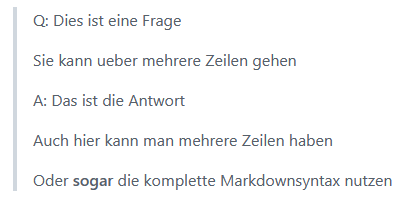
\includegraphics[width=50mm]{./figures/GH_Syntax1} & 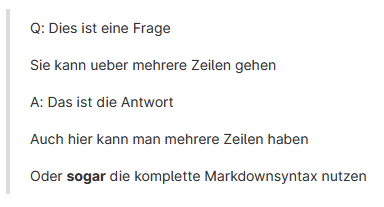
\includegraphics[width=50mm]{./figures/GL_Syntax1} & 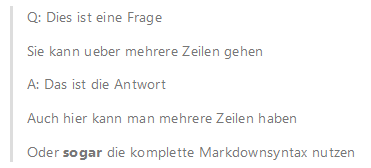
\includegraphics[width=50mm]{./figures/HD_Syntax1} \\
GitHub & GitLab & HedgeDoc \\
\end{tabular}
\caption{Rendering der in Abb. 1 definierten Syntax}
\end{figure}

Als Alternativansätze wurden folgende Syntaxmöglichkeiten betrachtet:

\paragraph{Durch Horizontallinien getrennte Karteikartenseiten:}~\\
Diese Syntax würde wiefolgt aussehen:
\begin{figure}[H]
\centering
\begin{lstlisting}
---
Q: Dies ist eine Frage

Sie kann ueber mehrere Zeilen gehen
---
A: Das ist eine Antwort

Auch hier kann man mehrere Zeilen haben

Oder **sogar** die komplette Markdownsyntax nutzen
---
\end{lstlisting}
  \caption{Ein Beispiel einer alternativen Karteikartensyntax}
\end{figure}

Während diese Syntax sehr leserlich in Markdownform und sehr einfach zu schreiben ist, hat sie mehrere Probleme.

Die Syntax kann nicht in der ersten Zeile benutzt werden, da sie Kollisionen mit der sogenannten Front Matter, ein auf YAML basierendes Metadatenformat innerhalb der Markdowndatei, hat. Front Matter wird sowohl von GFM, GLFM als auch HFM unterstützt.\\

Zudem ist es sehr einfach syntaktische Fehler zu machen, indem der Nutzer die letzte Horizontallinie weglässt.

Zuletzt ist das visuelle Rendering sehr unintuitiv, insbesondere da ohne freie Zeile die horizontale Linie in eine Überschrift umgewandelt wird

\begin{figure}[H]
\centering
\begin{tabular}{ccc}

\includegraphics[width=50mm]{./figures/GH_Syntax2} & 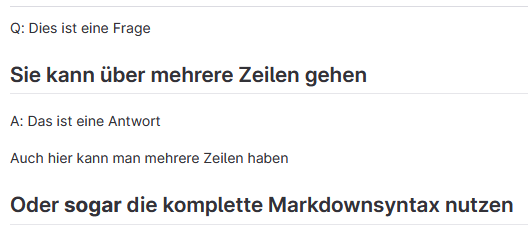
\includegraphics[width=50mm]{./figures/GL_Syntax2} & 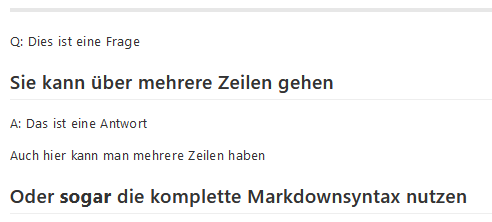
\includegraphics[width=50mm]{./figures/HD_Syntax2} \\
GitHub & GitLab & HedgeDoc \\
\end{tabular}
\caption{Rendering der in Abb. 3 definierten Syntax}
\end{figure}

\paragraph{Karteikarten in Tabellenform:}~\\
Diese Syntax würde wiefolgt aussehen:
\begin{figure}[H]
%\centering
  \begin{lstlisting}
| Question                       | Answer                              |
| ------------------------------ | ------------------------------------|
| Wofuer steht DFA?              | Deterministischer endlicher Automat |
| Welche Laufzeit hat Quicksort durchschnittlich? | O(n log n)         |
\end{lstlisting}
  \caption{Beispiel für eine tabellenbasierte Karteikartensyntax}
\end{figure}

Diese Syntax sieht gerendert sehr lesbar aus.

\begin{figure}[H]
\centering
\begin{tabular}{ccc}
  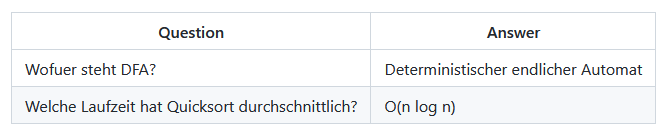
\includegraphics[width=0.5\textwidth]{./figures/GH_Syntax3} &
  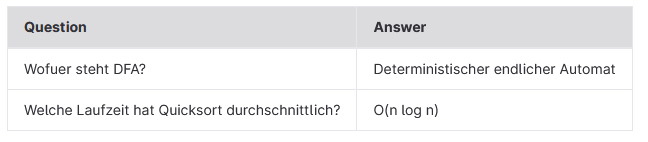
\includegraphics[width=0.5\textwidth]{./figures/GL_Syntax3}\\
GitHub & GitLab\\
\end{tabular}
  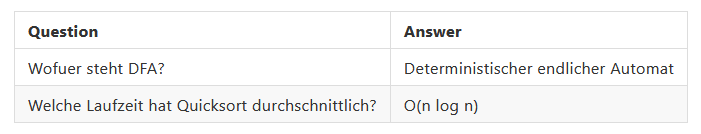
\includegraphics[width=0.5\textwidth]{./figures/HD_Syntax3} \\
  HedgeDoc
\caption{Rendering der in Abb. 5 definierten Syntax}
\end{figure}

Jedoch hat auch diese Syntax einige Nachteile. Zuerst eignet sich diese Syntax nicht für die Anwendung durch Literate Programming, da hierdurch nur viele einzeilige Tabellen zwischen dem Paragraphen entstehen würden. Zudem ist diese Art von Syntax sehr aufwändig für den Endnutzer, sofern dieser kein WYSIWYG-Editor nutzt. Zuletzt ist es weder möglich, eine Antwort über mehrere Zeilen zu definieren, noch sinnvoll Bilder einzubinden.

\paragraph{Karteikarten durch XML-Objekte:}~\\
Diese Syntax würde wiefolgt aussehen:
\begin{figure}[H]
\centering
\begin{lstlisting}
<anki>
  <q>
    Dies ist eine Frage

    Sie kann ueber mehrere Zeilen gehen
  </q>
  <a>
    Dies ist die Antwort

    Auch hier kann man mehrere Zeilen haben

    Oder sogar die komplette Markdownsyntax nutzen
  </a>
</anki>
\end{lstlisting}
  \caption{Beispiel für eine XML-basierte Karteikartensyntax}
\end{figure}

Der Inhalt hiervon wird leider von GitHub gar nicht gerendered, weswegen es für unseren Anwendungsfall nicht nutzbar ist. In GitLab und HedgeDoc werden die Tags nicht angezeigt, jedoch ist der Inhalt noch sichtbar.

\subsection{Unterst\"utzung von \LaTeX-Formeln}
Die Desktopversion von Anki ermöglicht bereits die Darstellung von \LaTeX-Formeln in Karteikarten. Hier wird beim ersten Anzeigen einer Karteikarte ein Bild der Formel mit einer lokal installierten \LaTeX-Engine gerendert und in der Anki-eigenen Mediendatenbank gespeichert. Die Formel in der Karteikarte wird durch das gerenderte Bild ersetzt. Somit muss jede Formel nur einmal gerendert werden. Insbesondere wird die Mediendatenbank über die Cloud synchronisiert. Somit reicht es, dass das erste Gerät eine \LaTeX-Installation hat.\\

Die Mobilappliaktionen wie AnkiDroid oder die iOS-Version haben jedoch keine Unterstützung für \LaTeX. Dies stellt normalerweise kein Problem dar, da bei der Karteikartenerstellung über die Desktopapplikation bereits die Formel gerendered wird. Da der Karteikartengenerator hier jedoch eigenständig zu Anki funktioniert, muss in Rahmen dieser Applikation auch die Formelgeneration übernommen werden.\\

Die Formelumwandlung ist jedoch nicht trivial. Das Problem hierbei sind die unterstützten Ausgabeformate:
\begin{itemize}
  \item \textbf{Portable Document Format (PDF):} PDF ist ein sehr komplexes Dateiformat. Es hat viele, sehr umfangreiche Standards und wird von nur wenig Applikationen korrekt implementiert. Somit ist die Rasterisierung von PDF von Applikationen sehr fehleranfällig.
  \item \textbf{Device independent file format (DVI):} DVI ist ein selten genutztes, obskures Seitenformat. \LaTeX ist die einzige große Applikation, welche noch DVI als Ausgabeformat unterstützt, da Knuth es als formell unterstütztes Ausgabeformat von \TeX definierte. Dementsprechend wenig Applikationen unterstützen DVI.
  \item \textbf{Encapsulated PostScript (EPS):} EPS ist ein für Drucker entwickeltes Vektorgrafikformat. Somit unterscheidet es sich sowohl von der Funktionalität als auch von der Nutzerschaft stark von pixelbasierten Bildformaten wie PNG.
\end{itemize}

Im folgenden wird eine Taxonomie der Konvertierungmöglichkeiten präsentiert:
\begin{itemize}
  \item \textbf{ImageMagick:} ImageMagick \cite{ImageMagick} ist ein Open-Source-Programm zur Bearbeitung von Raster- und Vektorgrafiken. Dieser Ansatz ist auch die etablierte Lösung des \TeX-Stackexchange \cite{TeXStackexchange}. Sie ist simpel, hat jedoch zwei Nachteile. Einerseits benötigt man sowohl \LaTeX als auch ImageMagick als externe Abhängigkeit; andererseits benötigt sie manuelle Anpassungen der Sicherheitsrichtlinien, was root vorraussetzt.
  \item \textbf{PDFium:} PDFium \cite{PDFium} ist die C++ PDF Bibliothek von Chromium \cite{Chromium}. Da man hierfür jedoch den kompletten Chromium-Browser benötigt, ist der Aufwand zu hoch. Die Kompilation von Chromium benötigt mindestens 8GB RAM sowie 100GB Festplattenspeicher zur Kompilation und braucht auf älterer Hardware mehrere Stunden.
  \item \textbf{KaTeX:} KaTeX \cite{KaTeX} ist eine in Javascript geschriebene \LaTeX-Implementation, welche auf Webseiten eingebunden werden kann um Formeln darzustellen. Sie wird unter anderem auch von GitHub und GitLab genutzt. Jedoch würde dies eine LaTeX-Engine wie Deno \cite{Deno} oder Node.js \cite{Node} vorraussetzen, welche sehr komplex einzubinden wäre.
  \item \textbf{dvisvgm:} Zuletzt gibt es \texttt{dvisvgm} \cite{dvisvgm}, welches PDF, DVI und EPS-Dokumente in SVG-Vektorgrafiken umwandeln kann. SVG ist das häufigst genutzte Vektorgrafikformat, für welches viele triviale PNG Konvertierungsmöglichkeiten existieren.
\end{itemize}

In unserem Fall haben wir uns für \texttt{dvisvgm} entschieden. Es ist eine Laufzeitabhängigkeit, jedoch in jeder kompletten TeXLive- sowie MikTeX-Installation vorhanden. Dies bedeutet, dass wir keine Abhängigkeiten haben, welche nicht auch von Anki vorrausgesetzt werden. Die von \texttt{dvisvgm} erstellen SVG-Grafiken werden dann durch \texttt{resvg} \cite{resvg} zu PNG exportiert.\\

Als Syntax wurde sich \texttt{\$\$f(x)=x\$\$} für \LaTeX entschieden\footnote{Um das Parsing simpel zu halten restriktieren wir diese Syntax vorerst nur auf einzelne Zeilen.}. Dies entspricht auch der KaTeX-Syntax, welche sowohl von HedgeDoc, als auch von GitHub oder GitLab genutzt wird.

\subsection{Commitbasierte Kartengeneration durch Continuous Integration (CI)}
Im Rahmen der Continuous Integration (CI) Softwarepraktik bieten alle großen Git-Repository-Hostinganbieter sogenannte Workflows an. Hierbei wird zu spezifischen Events wie Commits oder Pull Requests ein Container ausgeführt, welcher automatisiert vordefinierte Aufgaben erfüllen kann. Unter den typischen Aufgaben von CI zählen das Analysieren von Source Code nach Best-Practises, dem sogenannten Linting, der Ausführung automatisierter Tests sowie der Erstellung von Kompilaten.\\

In unserem Fall ermöglichen wir durch die Nutzung von CI-Workflows eine automatische Erstellung von Ankidecks aus Gitrepositories. Dieser Anwendungszweck ist so konzipiert das die Nutzerschaft gemeinsam kollaborativ via Git eine Ordnerstruktur an Anki-Markdowndokumenten erstellt. Im Rahmen dieses Praktikums wurden sowohl für GitLab \cite{GitlabTemplate} als auch für GitHub \cite{GithubTemplate} Repositoryvorlagen erstellt. Im folgenden wird ohne Beschränkung der Allgemeinheit die Funktionsweise anhand von Gitlab vorgestellt:

\begin{enumerate}
  \item Ein Nutzer macht eine Änderung an dem Repository und pusht den Commit auf den GitLab-Server. Die GitLab-Instanz startet einen OCI-Ubuntucontainer welcher das Repository im current working directory (CWD) eingebunden hat.
  \item Das System wird via \texttt{apt} aktualisiert und es werden folgende Abhängigkeiten installiert:
    \begin{itemize}
      \item curl (Zur Installation von Rust via \texttt{rustup} benötigt)
      \item git (Für den Download des Konvertierungsprogramms benötigt)
      \item \LaTeX (Zur Darstellung von Formeln zur Laufzeit benötigt)
      \item C-Compiler via \texttt{build-essential} (Zur Kompilation benötigt)
      \item pkg-config (Zur Kompilation benötigt)
      \item OpenSSL (Zur Kompilation benötigt)
      \item Rust-Compiler (Zur Kompilation benötigt)
    \end{itemize}
  \item Das Konvertierungsprogramm wird in das CWD via git gecloned und kompiliert.
  \item Das kompilierte Programm wird auf den Ordner mit den Anki-Markdowndokumenten angewandt.
  \item Das resultierende Karteikartenarchiv wird als Artifact den Nutzern bereitgestellt.
\end{enumerate}

\section{Funktionsweise}
Die Funktionweise ist in mehrere, disjunkte Schritte aufgeteilt, welche im folgenden betrachtet werden:
\begin{enumerate}
  \item \textbf{Markdownkarteikarten einlesen:} Innerhalb des per Programmargument übergebenen Pfades wird rekursiv nach allen Dateien gesucht, welche eine \texttt{.anki.md} Dateiendung haben. Alle gefundenen Dateien werden eingelesen und Karteikarten werden alle nach vorherig definierter Syntax extrahiert.
  \item \textbf{Formeln durch Bilder ersetzen:} Um die Mobilunterstützung zu sichern werden bereits zur Erstellung der Decks alle \LaTeX-Formeln zu PNG-Bildern umgewandelt, die dann in normaler Markdownsyntax als Ersatz der Formel eingesetzt werden.
  \item \textbf{Bilder lokal speichern:} Um die Möglichkeit der Offlinenutzung zu ermöglichen, werden sämtliche extern referenzierten Bilder lokal gespeichert.
  \item \textbf{Markdownkarteikarten in HTML umwandeln:} Mit der \texttt{comrak}-Bibliothek \cite{comrak} werden die Markdownkarteikarten in äquivalente HTML-Dokumente umgewandelt.
  \item \textbf{HTML-Karteikarten und Bilder in Anki-Archiv speichern:} Die generierten Karteikarten werden nun als Ankideckarchiv gespeichert. Die interne Struktur entspricht hierbei der genutzten Ordnerstruktur.
\end{enumerate}
\section{Diskussion}
\subsection{Audio- und Videounterst\"utzung}
Diese Version unterstützt weder Audio- noch Videoeinbettung. Hierfür gibt es zwei Gründe:
\begin{enumerate}
  \item \textbf{Schlechte Anki-Unterstützung:} Offiziell ist die Einbettung von Audio- und Videodateien in Anki-Karteikarten möglich, jedoch ist der Support dafür nicht adäquat. Wenn Audiodateien ohne weitere Anpassungen eingebunden werden, starten sie direkt nach dem initialen Laden der Karte, ohne das Steuerungsmöglichkeiten zum Pausieren oder zur Lautstärkeeinstellung vorhanden sind. Bei Videodateien öffnet sich ein zusätzliches Pop-up-Fenster, das einen mpv-Player startet und das Video automatisch abspielt. Diese Probleme kann man jeodoch umgehen, in dem man manuell die HTML-Elemente in die Karte integriert und die Medien nur indirekt referenziert. Im Rahmen dieser Arbeit wurde auch ein Proof of Concept diesbezüglich erstellt \cite{AnkiPoC}.
  \item \textbf{Keine native Markdownunterstützung:} Weder CommonMark noch GFM\footnote{GFM unterstützt Videos, jedoch nur in Pull Requests und Issues \cite{GFMVid}.} oder GLFM definieren einen offiziellen Weg Audio- und Videodateien einzubinden. HedgeDoc bietet nur die Möglichkeit für YouTube- oder Vimeovideos \cite{HFM2}. Keiner der genannten Standards unterstützen Audiodateien. Somit gibt es keinen kanonischen Weg Video oder Audio syntaktisch sinnvoll einzubinden.
\end{enumerate}
\subsection{Geplante Weiterentwicklung und Einsatz der Software}
Obwohl die erste Version erfolgreich entwickelt wurde, gibt es noch einige geplante Folgeentwicklungen:

\begin{itemize}
  \item Die Anki Markdown-Spezifikation sollte erweitert werden, um mehr Medientypen auf eine kompatible Weise abzudecken. Dies sollte in einem offenen, RFC-ähnlichen Prozess geschehen, wo alle Interessen- und Nutzergruppen einbezogen werden.
  \item Die Anwendung sollte auch für Nicht-Informatiker zugänglicher werden. Dies bedeutet die Entwicklung einer Benutzeroberfläche und die Erschaffung einer insgesamt einfacheren Benutzererfahrung. Außerdem sollte eine angemessene Dokumentation erstellt werden, worin viele WYSIWYG-Tools für die Erstellung von Flashcards vorgestellt werden sollten.
\end{itemize}

Neben diesem Punkten ist geplant, sowohl mit der Fachgruppe Informatik sowie einer Anki-Projektgruppe eines Medizinstudentenvereins Testläufe zu gestalten, in welchen iterativ die Software und die dazugehörigen Arbeitsprozesse verbessert werden.
\newpage
\section{Literaturverzeichnis}
\printbibliography
\end{document}
